标签感知推荐系统是当前推荐系统研究的一个研究热点,其研究内容主要分为数据和算法两个方面。在数据部分,最为关键的是如何准确地定义社会标签数据,并将其有效地融入到标签感知推荐算法中。社会标签数据的定义对于整个推荐系统至关重要。算法部分则负责从社会标签数据中学习到用户、标签、物品的表征,并将其运用到最终的推荐环节中,为用户提供个性化的推荐服务。

\section{社会标签数据}
社会标签数据是指用户在社交网络和互联网等平台上由用户自主添加的标签信息。社会标签数据以其丰富的语义信息和用户生成的特点,成为推荐系统中重要的数据来源之一。本节将重点介绍标签感知推荐系统中常用的社会标签数据建模方式,并对社会标签数据的建模定义进行详细讲解。
\subsection{社会标签的研究}
社会标签数据是标签感知推荐系统实现个性化推荐的关键基础。社会标签数据被广泛应用于解决用户和物品之间信息缺失的问题,从而更加准确地描述用户的偏好和物品的特征\cite{hutchison_information_2006, bischoff_can_2008}。这些社会标签的数据是通过标签感知推荐系统中的大众分类工具(即 Folksonomy)进行积累的。该工具允许用户对他们所交互的物品(例如电影、音乐和书签)自由地进行标注。由此组成的社会标签数据是由简明扼要的单词或短语组成,可以反映单个用户的观点,同时也可以获得大众集体智慧的评价。从这个角度来看,社会标签数据中的标签可以作为用户和物品之间交互的桥梁。通过对社会标签数据的探索,标签感知推荐系统可以为用户提供精确的个性化 Top-K 推荐结果 \cite{zuo_tag-aware_2016,li_tag-aware_2019,chen_tgcn_2020}。因此,将社会标签数据引入推荐系统可以提高推荐的质量,同时在一定程度上提高推荐系统的可解释性。

在标签感知推荐系统中,如何准确地定义和处理社会标签数据是实现个性化推荐的基础。常用的社会标签数据建模方式包括基于用户的标签建模、基于物品的标签建模和基于标签的用户-物品关联建模等。其中,基于用户的标签建模主要是通过对用户行为数据的分析,从中提取出用户与标签之间的关系,并构建<用户-标签>的映射关系;基于物品的标签建模则是针对不同物品之间的标签差异进行建模,从而分析物品与标签之间的关系;而基于标签的<用户-物品>关联建模则是将标签作为桥梁,分析用户和物品之间的关系。
% 例如,CFA\cite{zuo_tag-aware_2016} 使用一个稀疏的自动编码器来获取基于标签的用户潜在表征,并与基于用户的协同过滤相结合。此外,DSPR\cite{xu_dspr_2016} 和 HDLPR\cite{xu_hdlpr_2017}利用多层感知器来处理这种稀疏的特征向量并提取抽象的用户和项目表征。AIRec\cite{chen_airec_2021} 提供了一个带有分层注意力网络的混合用户模型,它可以从显性的用户分类记录中描绘用户的隐性偏好。

尽管已有多种方法提高了标签感知推荐算法的推荐性能,但由于数据的稀疏性和标签的一次多义性与多词同义性,推荐系统仍然面临一些无法接受的问题\cite{shepitsen_personalized_2008}。稀疏性指大多数用户只为他们少数交互过的物品标注标签,导致标签数据不够充分。一次多义性和多词同义性的问题来自于上下文信息的缺失以及用户表达习惯的不确定性。图~\ref{fig:tags}~展现了一些例子。一些具有不同形式的标签有着相同的含义,图中的 “第二次世界大战” 和 “二战” 在社会标签数据中是不同的标签,但通常被不同的用户分配给同一部电影 “辛德勒的名单”。另一些相同的标签却有着不同的含义,图中的 “苹果” 在科技爱好者群体当中,会被视为是一家科技公司,但大多数人则认为它是一种水果。

\begin{figure}[!h]
    \centering
    \setlength{\belowcaptionskip}{-6mm}
    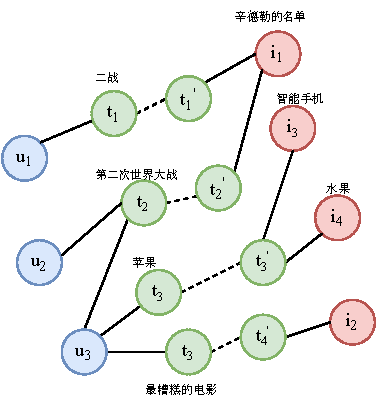
\includegraphics[width=0.4\linewidth]{figure/tags.drawio.pdf}
    \caption{用户、标签与物品}
    \label{fig:tags}
\end{figure}

本文针对社会标签数据进行了建模定义,提出了一种基于标签的用户-物品关联建模方法。具体而言,通过对用户在社交网络平台中添加的标签进行分析,提取出用户和标签之间的关系,并将其映射到用户-标签矩阵中,以此构建起用户-标签图;同时,通过对物品的标签进行分析,提取出物品与标签之间的关系,并将其映射到物品-标签矩阵中,以此构建起物品-标签图。在此基础上,通过对用户-标签图和物品-标签图进行分析,建立起基于社会标注图,从而实现对用户个性化需求的精准推荐。

\subsection{社会标注图}
本文研究标签感知推荐系统中,利用大众标注记录的两种主要方式。目前主要存在两种方法,一种是将标签编码成隐向量的形式\cite{zuo_tag-aware_2016,chen_airec_2021},另一种是构建包含多种关系的异构图\cite{chen_tgcn_2020}。
本文与上述方法不同之处在于,利用大众标注记录中的 $a=(u,t,i) \in \mathcal{A}$ 两组边 $\mathcal{E}_{u,t}$ 和 $\mathcal{E}_{i,t}$ 构建了两个含义不同的二部图。其中,集合 $\mathcal{E}_{u,t}$ 表示用户主动标注标签的行为,而集合 $\mathcal{E}_{i,t}$ 表示物品被动接受标签的行为。在标签感知推荐系统当中,集合 $\mathcal{E}_{u,t}$ 和 $\mathcal{E}_{i,t}$ 中的边可以被定义为:
\begin{gather}
    e_{u,t} = 
    \begin{cases}
        1,&\text{if $(u,t) \in \mathcal{E}_{u,t}$} \\
        0,&\text{otherwise}
    \end{cases},
\end{gather}
\begin{gather}
    e_{i,t} = 
    \begin{cases}
        1,&\text{if $(i,t) \in \mathcal{E}_{i,t}$} \\
        0,&\text{otherwise}
    \end{cases}.
\end{gather}

基于上述边的定义,本文可以根据整个社会标注数据 $\mathcal{A}$,构建一个社会标注图。该图由用户-标签的标注行为和物品-标签的被标注行为组成。每种边的集合可以使用两个二部图 $\mathcal{G}_{UT} = (\mathcal{U}, \mathcal{T}, \mathcal{E}_{u,t})$, $\mathcal{G}_{IT} = (\mathcal{I}, \mathcal{T}, \mathcal{E}_{i,t})$ 来表示。

\section{标签感知推荐算法}
推荐系统是一个涉及计算机科学、心理学、社会学等多个学科领域的综合性问题,包含了许多内容。然而,推荐算法的模型可以被抽象为“学习推荐”(learning to recommend)的问题。在这个问题中,我们的目标是学习一个模型,该模型可以根据用户历史行为和物品属性等信息,预测用户可能喜欢的物品并向其进行推荐。本节将介绍如何对标签感知推荐算法进行数学建模。

推荐系统是一个涉及多个学科领域,如计算机科学、心理学和社会学等的广泛领域。推荐算法的模型可以被抽象为“学习推荐”的问题。在此背景下,本节介绍如何将标签感知推荐算法数学化。标签感知推荐算法的问题可以抽象为学习预测函数 $f$。该函数以社会标签数据 $\mathcal{A}$ 中用户$u$ 的信息集合 $\mathcal{U}$ 、物品 $i$ 的信息集合 $\mathcal{I}$ 和标签 $t$ 的信息集合 $\mathcal{T}$ 作为输入,输出预测分数 $\hat{y}$,表示用户与物品之间发生交互的概率,$f: \mathcal{U} \times \mathcal{T} \times \mathcal{I}$。接着,对每个用户候选物品按交互概率从高到低排列,从中选择 $K$ 个物品组成用户的个性化推荐列表,这一任务被称为 Top-K推荐任务。根据所使用的数据方式不同,现有的推荐算法研究可以划分为基于协同过滤的方法和基于富信息的方法\cite{wu_survey_2022}。两者的区别在于,基于协同过滤的方法通常只使用用户和物品信息中的 ID 特征,即用户在推荐系统中的唯一标识,而基于富信息的方法则会引入如用户性别、用户年龄、物品评论等信息。与之前将标签信息作为富信息的方法不同\cite{zuo_tag-aware_2016,xu_dspr_2016,chen_airec_2021},本文主要探讨基于协同过滤方法,仅使用标签的 ID 特征而不考虑标签内容,即:
\begin{gather}
    \hat{y}_{ui} = f(u, i, t),
\end{gather}
在构建了推荐模型之后,通常会使用优化目标函数来优化推荐模型的参数,即:
\begin{gather}
    \mathop{min}_{\Theta} ~ \mathop{\mathbf{E}}_{\mathcal{A}^+} ~ \mathcal{L}(f),
\end{gather}
其中,$\mathcal{L}(\cdot)$ 是定义在 $f$ 上的损失函数,$\mathcal{A}^+$ 是观测到的社会标签数据集合,$\Theta$ 是模型参数。

由于本文专注于为标签感知推荐系统中用户提供个性化推荐列表。通过“学习推荐"得到推荐模型后,标签感知推荐系统将会生成Top-K推荐列表:
\begin{gather}
    Top(u, K) = \mathop{argmax}^{(K)}_{i\in \mathcal{I}}\hat{y}_{u,i}.
\end{gather}

\section{本章小结}
本章探讨了标签感知推荐系统数据和算法两个方面。在数据部分,本章梳理了构建标签数据的研究现状,并基于现有研究的缺陷给出了社会标注图的定义。在算法部分,本章给出了标签感知推荐系统的模型构建和优化目标的形式化定义。